Estimating depth from images is an important open problem with applications to robotics, autonomous driving, and medical imaging. Dense depth maps are useful precursors to higher-level scene understanding tasks such as pose estimation and object detection.

Depth sensing is vital for the success of many computer vision tasks, such as navigation~\cite{geiger2013vision}, robotic vision, semantic segmentation~\cite{ren2012rgb,silberman2012indoor,gupta2013perceptual}, 3D object detection~\cite{shrivastava2013building,lin2013holistic,gupta2014learning,song2014sliding,song2016deep}, and 3D object classification~\cite{wu20153d,maturana2015voxnet,qi2016volumetric}. However, traditional depth sensing techniques require multiple cameras, active illumination, camera motion, or other aspects that may make their deployment challenging.

One of the most promising approaches to overcoming these challenges is monocular depth estimation (MDE)~\cite{Saxena2006,Eigen2014,Laina2016,Fu2018,Alhashim2018}. Given a single RGB image, a monocular depth estimator uses pictorial cues in the image, such as perspective, occlusion, shading, and relative object size, to predict a dense depth map of the scene. While neural networks solving the MDE problem have significantly improved over the last years, this remains an ill-posed inverse problem with inherent scale ambiguity. Pictorial cues alone allow for the ordinal depth, that is the relative ordering of objects in a scene, to be robustly estimated~\cite{Eigen2014,Fu2018}. However, MDE approaches to date are incapable of reliably estimating absolute distances of a scene. Interestingly, Alhashim and Wonka~\cite{Alhashim2018} recently showed that if the MDE network has oracle access to the ground truth median scene depth, then correcting the output of the estimator to match this median depth produces accurate absolute depth maps.

%For example, a larger object at a far distance to the camera results in the same 2D camera image as a smaller object of the same type that is closer to the camera. Therefore, MDE approaches to date are incapable of reliably estimating absolute distances of a scene. Interestingly, Alhashim and Wonka~\cite{Alhashim2018} recently showed that if the MDE network has oracle access to the ground truth median depth, then correcting the output of the CNN to match this median depth produces accurate absolute depth maps both qualitatively and quantitatively.

% move to discussion
%However, traditional approaches to depth estimation, such as stereo, suffer from lower performance when confronted with small angles or faraway objects. More exotic approaches use FMCW or time-of-flight LiDAR technologies, but these approaches are currently expensive and bulky. 

%The most promising solution to these issues uses deep learning and convolutional neural networks to perform \textit{monocular depth estimation}, estimating dense depth maps from single RGB images.  However, this problem is underconstrained due to \textit{inherent scale ambiguity}, the unresolvable tradeoff between size and distance in single images. In practice, this issue commonly manifests itself in many monocular depth networks, and indeed, Wonka et. al. (cite) showed that if the method has oracle access to the ground truth median depth, then correcting the output of the CNN to match this median depth produces better depth maps both qualitatively and quantitatively.

\begin{figure}
  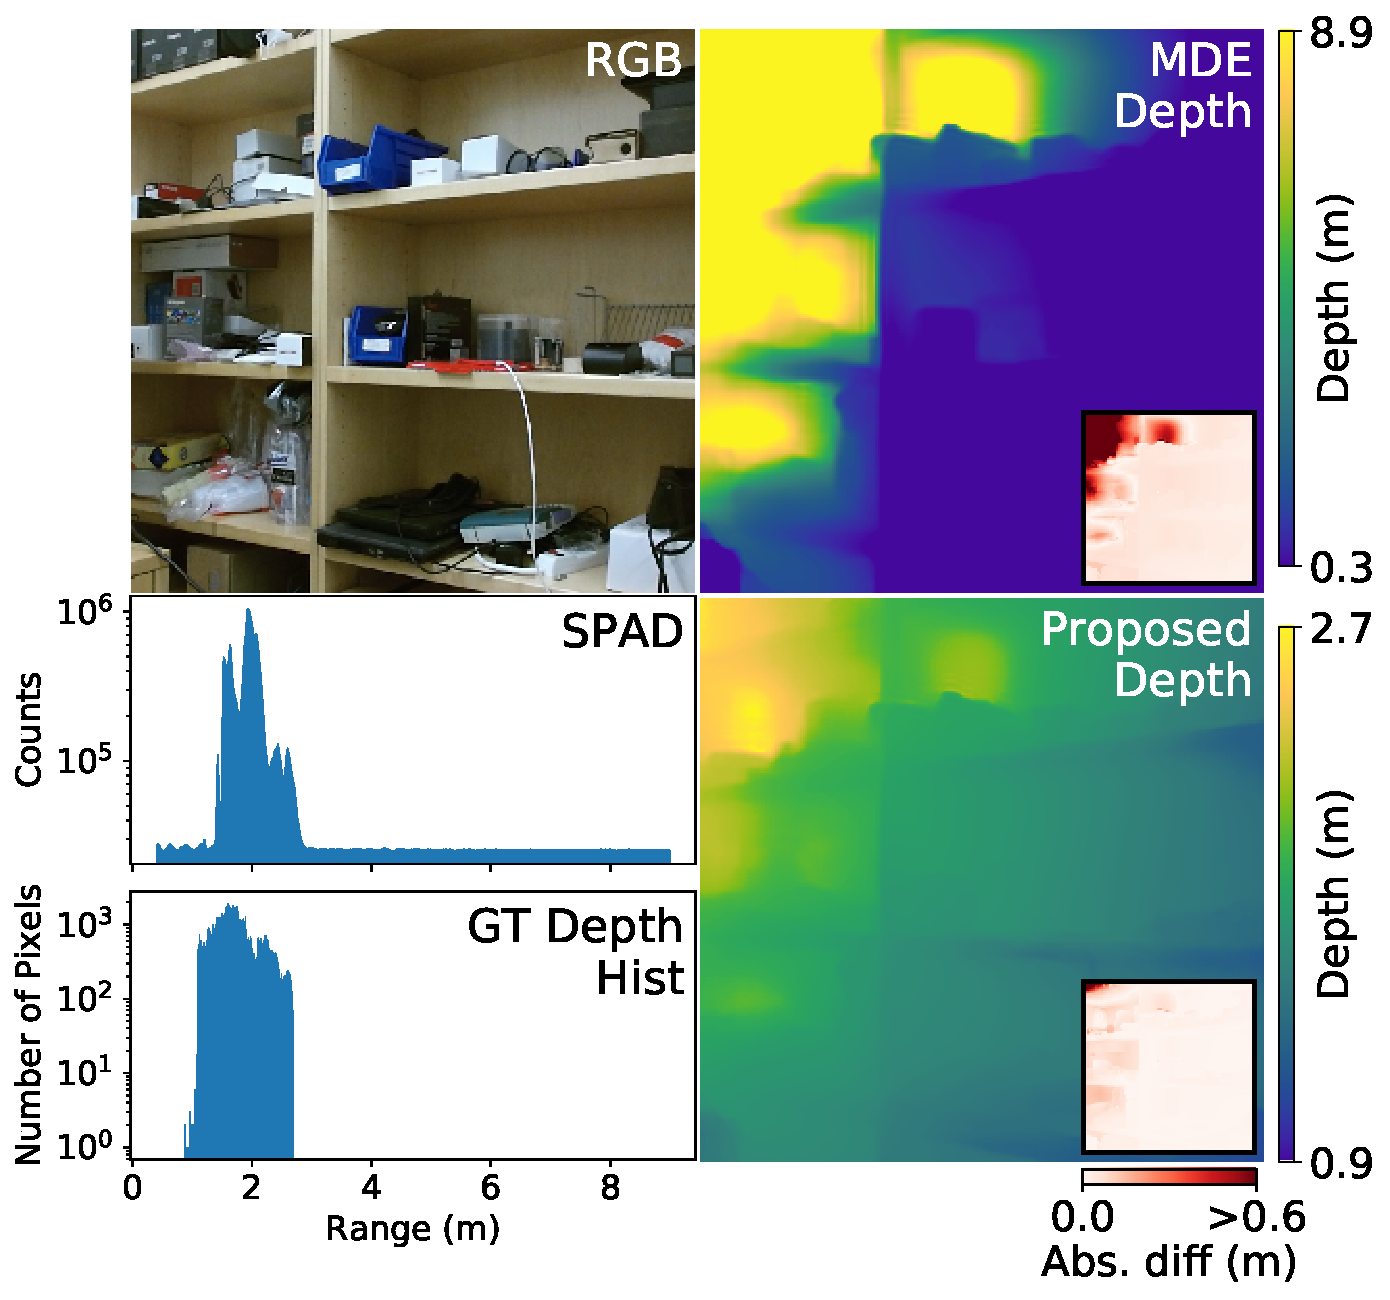
\includegraphics[width=\linewidth]{teaser.pdf}
  \caption{Monocular depth estimation predicts a depth map (upper right) from a single RGB image (upper left). Unfortunately, this is an ill-posed problem subject to ambuguity that prevents reliable absolute depth estimation (error, inset image). The proposed method uses the transient measured by a diffused SPAD (lower left), which closely resembles the shape of a histogram of the ground truth depth map, to correct the output of the depth estimation and optimize the quality of the estimated absolute depth.}
  \label{fig:teaser}
\end{figure}

While access to ground truth depth is impossible in a realistic scenario, one of our primary insights is that low-cost sensors capable of capturing aggregated depth information of a scene are readily available and already part of the sensor suite of many cellphones. These proximity sensors, for example deployed in Apple's iPhones, contain a low-power pulsed light source and a single-pixel, single-photon avalanche diode (SPAD) to sense the distance of one ray direction in front of the camera. Coupled with high-power laser sources, SPADs also form the backbone of emerging single-photon LiDAR systems~\cite{Kirmani:2014,pawlikowska2017single,Li:2019}. Whereas individual SPADs are easy to fabricate and sufficiently cost effective to be deployed in consumer electronics, the required ultra-fast time-stamping electronics make it difficult to fabricate high-resolution SPAD arrays at low cost. A single or a few SPADs could certainly be used together with a raster scanning mechanism, which is typical for LiDAR systems, but the mechanical complexity of such a system prevents usage in mobile devices and the inherent tradeoff between scan speed and resolution makes it difficult to capture high-resolution depth maps at high framerates.

Here, we propose to use a single-pixel SPAD and pulsed light source in an unconventional way. Rather than optically focusing them to record the distance along one ray, we diffuse the emitted light and the detector over the entire scene. This allows us to directly capture the integrated depth of the scene---a depth histogram. Technically, a diffused SPAD does not record a true depth histogram but a transient that is affected by square-distance falloff of the backscattered light, spatially varying reflectance of the scene, ambient photons, and detector noise. However, we can interpret the measurements of a single-pixel SPAD as something similar to a depth histogram while keeping in mind that they are not exactly the same.

%In this paper, we go further and show that by augmenting the RGB image with a histogram of global image depths, we can achieve substantially improved performance (and generalizability) over state-of-the-art monocular depth estimators. By performing an exact, weighted histogram matching on the output depth map of the depth estimator, we can match the depth histogram of the scene to the depth histogram of our estimate. This histogram matching is described in (cite) and is flexible enough to accommodate different pixel reflectances in the RGB image. Finally, this histogram can be captured relatively inexpensively using only a single pixel single-photon avalanche diode (SPAD) and pulsed laser illumination diffused over the field of view, representing a significant improvement in cost and simplicity over multi-pixel LiDAR arrays with expensive scanning mechanisms. It is worth noting that SPADs of this type have already made their way into existing smartphones, such as the iPhone X, and will likely play a role in future mobile sensing platforms as well.


% move to discussion
%Our method is not without limitations. It still requires a laser and single-pixel LiDAR detector, and as such, is sensitive to ambient photons. Being  a variant of histogram matching, our method is unable to transpose the values of pixels (i.e. if pixel $a$ is farther than pixel $b$ in the input, it will be farther than pixel $b$ in the output). In other words, our method is not able to resolve ordinal depth errors (errors where an object is wrongly placed closer or farther relative to another object). Finally, our method is non-differentiable, and is therefore unsuitable for end-to-end optimization of multi-part networks.

In this paper, we develop a sensor fusion strategy that processes the ordinal depth computed by some monocular depth estimator to match the output of the diffused SPAD. With extensive simulations, we demonstrate that our approach achieves substantial improvements in the quality of the estimated depth maps, comparable to the oracle median depth, disregarding which specific depth estimator is used. Moreover, we build an RGB-SPAD camera prototype and again demonstrate that our sensor fusion strategy achieves significantly higher-quality depth maps for a variety of captured scenes than a monocular depth estimator alone. With this work, we present a practical way to disambiguate depth estimation with RGB images using minimal additional sensing hardware. Specifically, we make the following contributions:
%
\begin{itemize}
	\item We introduce the idea of augmenting an RGB camera with a global depth histogram captured by a SPAD to address scale ambiguity error in monocular depth estimators.	
  \item We analyze this approach on indoor scenes using the NYU Depth v2 dataset and demonstrate that our approach is able to resolve scale ambiguity while being fast and easy to implement.
	\item We build a prototype RGB-SPAD camera and evaluate its efficacy on captured data, assessing both the quality and the ability of our method to help generalization of monocular depth estimators across scene types. 
\end{itemize}


